\section{Fuzzing Fundamentals}
\label{sec:ff}

Since it was first proposed in 1990 \cite{miller1990empirical}, fuzzing has established itself as a standard method for automated vulnerability detection. At its core, fuzzing involves the iterative generation of malformed test cases to explore the input space of an application with the aim of triggering unintended program behaviour. 

The assumption is that if an application's input validation cannot gracefully handle unexpected inputs, those inputs may expose vulnerabilities. Various fuzzing techniques have been proposed \cite{aschermann2019nautilus, chen2018angora, dutra2023formatfuzzer}, developed \cite{honggfuzz, libfuzzer, zalewski2014afltech}, and used effectively to identify a large number of vulnerabilities \cite{honggfuzzbugs, syzkallerbugs, rashbugs}.

\subsection{Components of a Fuzzer}

While fuzzing techniques can vary widely in their implementation, most modern fuzzers share a common set of basic entities \cite{fioraldi2022libafl}.

\paragraph{Input} The fuzzer's internal representation of data, which may differ from the format the program actually consumes. Simple fuzzers manipulate input as raw bytes, while more advanced engines work with more complex structures --- such as Abstract Syntax Trees \cite{aschermann2019nautilus} or system calls \cite{syzkaller} --- to modify the data while maintaining its validity. 

\paragraph{Corpus} A fuzzer's corpus stores inputs and their metadata, typically either in memory or on disk. Fuzzing models generally require at least two corpora: one used to evolve interesting test cases, and another for saving successful solutions (i.e., crashes).

\paragraph{Scheduler} Strictly tied to the corpus, it determines which test cases should be evaluated next. Basic implementations might rely on a FIFO queue or random selection, while more complex schedulers use heuristics to prioritise more valuable inputs \cite{chen2020meuzz, rebert2014optimizing, wang2021reinforcement}.

\paragraph{Stage} A component that executes one or more specific actions --- such as mutation, analysis, or minimisation --- on a single test case.

\paragraph{Observer} An observer provides data from an execution of the target program, which is used to efficiently analyse the execution itself. A common example of an observer is the coverage map, although other types exist \cite{aschermann2020ijon, padhye2019fuzzfactory}.

\paragraph{Executor} The component responsible for actually executing the target, which defines all operations related to a single run of the target program with the given input. It can vary in complexity, from a call to a harness \cite{libfuzzer} to restarting an operating system from a snapshot \cite{schumilo2021nyx}.

\paragraph{Feedback} Feedback is used to classify the outcome of an execution as interesting or not. It processes the information given by one or more observers. 

\paragraph{Mutator} The mutator is responsible for generating new inputs through the transformation of one or more existing inputs. These operators can be random or format-aware, enabling them to manipulate the input's internal representation \cite{wang2019superion}.

\paragraph{Generator} A component designed to generate new inputs from scratch. It can be completely random or grammar-based \cite{aschermann2019nautilus}.

\begin{figure}
    \centering
    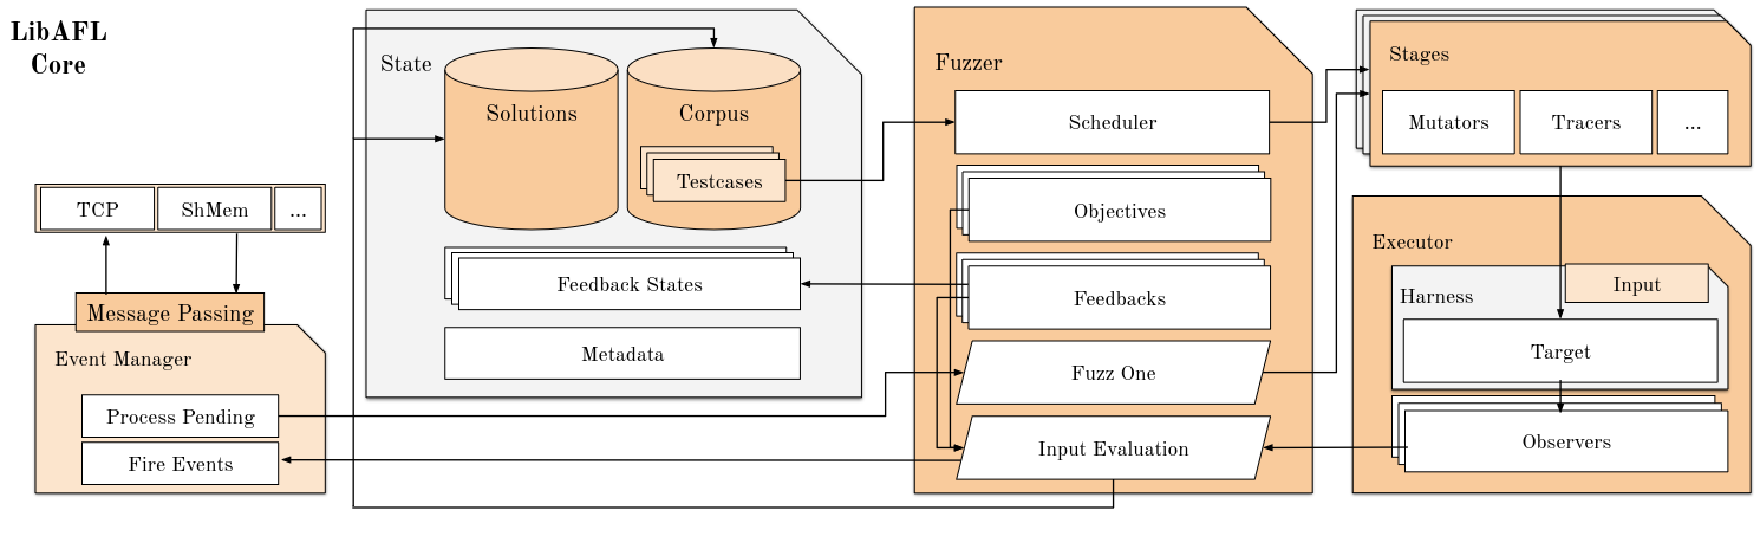
\includegraphics[width=\linewidth]{imgs/background/libaflcore.pdf}
    \caption{\textsc{LibAfl} core architecture, as shown in \cite{fioraldi2022libafl}, Figure 1}
    \label{fig:libaflcore}
\end{figure}

\subsubsection{Core Fuzzing Loop}

All feedback-driven fuzzers share a common core loop, which can be decomposed into four main stages:
\begin{enumerate}
    \item \textbf{Input generation and scheduling}: The scheduler chooses an input from the corpus to be passed on to the mutator.

    \item \textbf{Execution}: The new candidate input is injected into the target program, in a manner defined by the executor.

    \item \textbf{Feedback evaluation}: The information collected during execution is used to determine whether an input is interesting. The definition of ``interesting'' is abstract, but is always correlated with novelty in the search (e.g., new code or edge coverage).

    \item \textbf{Corpus update}: The set of interesting test cases and solutions is updated according to the feedback. The cycle then repeats.
\end{enumerate}

\subsection{Fuzzer Classification}

The taxonomy of fuzzers is traditionally established along two main criteria: the methodology for test case generation and the level of visibility into the target program.

\paragraph{Based on Input Generation} The first classification criterion relies on how test cases are produced, generally dividing fuzzers into two categories:
\begin{itemize}
    \item \textbf{Generation-based} fuzzers create new test cases from scratch, using a specification of the input format, e.g., a model \cite{peachfuzzer} or block \cite{aitel2002advantages}.

    \item \textbf{Mutation-based} fuzzers rely on a pre-existing corpus, which must be provided in the initial state.
\end{itemize}

\paragraph{Based on Target Knowledge} This criterion evaluates the extent to which a fuzzer can observe the internal state and execution paths of the target program. This traditionally divides fuzzers into three categories \cite{liang2018fuzzing}:
\begin{itemize}
    \item \textbf{Black-box} fuzzers treat the target application as an opaque system, interacting with it solely through input/output channels and observing external outcomes, such as crashes or hangs. These are closely related to random testing. However, a lack of information about the target's implementation does not imply a lack of specification knowledge; black-box fuzzers might still require a model of the input format to generate test cases.

    \item \textbf{White-box} fuzzers possess complete visibility of the target's internals, typically employing techniques such as symbolic execution to leverage constraints found during execution \cite{godefroid2008automated}.

    \item \textbf{Grey-box} fuzzers represent a middle ground, collecting minimal information to better explore the input space while limiting performance overhead. This feedback is typically based on code coverage and is collected through instrumentation \cite{zalewski2014afltech}.
\end{itemize}

\subsection{Coverage-Guided Fuzzing}

Empirical data \cite{ossfuzz} strongly suggests that integrating code coverage feedback into the fuzzing process increases overall efficiency, thereby yielding a higher number of faults discovered in a fixed time window.

There are many fuzzers that rely on code coverage as feedback, but the technique is not limited to this type of information \cite{aschermann2020ijon, wang2019sensitive}.

Fuzzers typically employ evolutionary algorithms to analyse execution feedback obtained from the target program, using this data to guide subsequent input generation. A general version of these algorithms is presented in Algorithm \ref{alg:evolfuzzing}.

\begin{algorithm}
\caption{Basic Evolutionary Fuzzing}\label{alg:evolfuzzing}
    \begin{algorithmic}[1]
    \State $F \gets \emptyset$ \Comment{Set of faults found}

    \State $S[C] \gets InitialCorpus$ \Comment{$S$ represents the fuzzer state}

    \While{\Call{ContinueFuzzing}{$S$}}
        \State $t \gets \Call{SelectTestcase}{S[C]}$ 
    
        \State $N \gets \Call{Calibrate}{t, S}$ \Comment{Determines time spent on $t$}
    
        \For{$i \gets 1$ \textbf{to} $N$}
            \State $t' \gets \Call{Mutate}{t}$ 
        
            \State $Tr \gets \Call{Execute}{T, t'}$ \Comment{Run target and obtain execution trace}

            \If{\Call{IsViolation}{$Tr, t'$}}
                \State $F \gets F \cup \{t'\}$
            \EndIf

            \If{\Call{IsInteresting}{$Tr, S$}}
                \State $S[C] \gets S[C] \cup \{t'\}$
            \EndIf
        \EndFor
    \EndWhile
    \Return{$F$}
\end{algorithmic}
\end{algorithm}

Code coverage is an abstract concept that, in the literature, is typically evaluated using one of three elements: basic blocks, basic block paths and, most commonly, basic block edges \cite{fioraldi2020afl++, honggfuzz, libfuzzer, zalewski2014afltech}. Tracking edges is the most common approach as it allows more granular tracking than simple block coverage, distinguishing between different traces spanning the same basic blocks, while avoiding problems such as path explosion.

For source-available binaries, code coverage is generally measured through instrumentation at compile time \cite{honggfuzz, zalewski2014afltech}. For source-unavailable binaries, feedback can be obtained via instrumentation inserted dynamically \cite{fioraldi2020afl++, rawat2017vuzzer}, or statically through binary rewriting \cite{dinesh2020retrowrite}.